\documentclass[12pt]{article} 
\usepackage[margin=2cm]{geometry} 
\usepackage{psfrag} 
\usepackage{graphicx} 
\usepackage{epstopdf} 
\usepackage{longtable,booktabs} 
\usepackage{amsmath,amsfonts} 
\usepackage{breqn} 
\usepackage{float,morefloats,caption} 
\begin{document} 
% 25-Jul-2024 16:08:32, created by McMCDiagnostics.m 
 
\begin{center}
\begin{longtable}{lcc} 
\caption{MCMC Inefficiency factors per block}\\
 \label{Table:MCMC_inefficiency_factors}\\
\toprule 
$Parameter                 $	 & 	 $     Block~1$	 & 	 $     Block~2$\\
\midrule \endfirsthead 
\caption{(continued)}\\
 \toprule \\ 
$Parameter                 $	 & 	 $     Block~1$	 & 	 $     Block~2$\\
\midrule \endhead 
\midrule \multicolumn{3}{r}{(Continued on next page)} \\ \bottomrule \endfoot 
\bottomrule \endlastfoot 
$ \sigma_{{e_x}}           $	 & 	      12.259	 & 	      12.388 \\ 
$ \sigma_{{e_{b}}}         $	 & 	     638.579	 & 	     661.602 \\ 
$ \sigma_{{e_{alpha,L}}}   $	 & 	     725.655	 & 	     736.597 \\ 
$ \sigma_{{e_{\delta}}}    $	 & 	     664.614	 & 	     663.912 \\ 
$ \alpha_L                 $	 & 	     525.841	 & 	     441.238 \\ 
$ b                        $	 & 	     726.369	 & 	     741.312 \\ 
$ \phi                     $	 & 	     594.042	 & 	     702.367 \\ 
$ {\delta}                 $	 & 	     740.854	 & 	     742.190 \\ 
$ {1/\xi}                  $	 & 	     698.780	 & 	     725.551 \\ 
$ {\rho_x}                 $	 & 	     172.471	 & 	     195.687 \\ 
$ {\rho_Z}                 $	 & 	     689.724	 & 	     725.420 \\ 
$ {\rho_{\alpha_L}}        $	 & 	     714.679	 & 	     733.778 \\ 
$ {\rho_N}                 $	 & 	      42.307	 & 	      49.828 \\ 
\end{longtable}
 \end{center}
% End of TeX file.
 
% 25-Jul-2024 16:08:55, created by stoch_simul.m 
 
\begin{center}
\begin{longtable}{lcccc} 
\caption{MATRIX OF COVARIANCE OF EXOGENOUS SHOCKS}\\
 \label{Table:covar_ex_shocks}\\
\toprule 
$Variables      $	 & 	 $            {e_x}$	 & 	 $          {e_{b}}$	 & 	 $    {e_{alpha,L}}$	 & 	 $    {e_{\delta}}$\\
\midrule \endfirsthead 
\caption{(continued)}\\
 \toprule \\ 
$Variables      $	 & 	 $            {e_x}$	 & 	 $          {e_{b}}$	 & 	 $    {e_{alpha,L}}$	 & 	 $    {e_{\delta}}$\\
\midrule \endhead 
\midrule \multicolumn{5}{r}{(Continued on next page)} \\ \bottomrule \endfoot 
\bottomrule \endlastfoot 
${e_x}          $	 & 	         0.000027	 & 	         0.000000	 & 	         0.000000	 & 	         0.000000 \\ 
${e_{b}}        $	 & 	         0.000000	 & 	         0.036834	 & 	         0.000000	 & 	         0.000000 \\ 
${e_{alpha,L}}  $	 & 	         0.000000	 & 	         0.000000	 & 	         0.018060	 & 	         0.000000 \\ 
${e_{\delta}}   $	 & 	         0.000000	 & 	         0.000000	 & 	         0.000000	 & 	         0.024591 \\ 
\end{longtable}
 \end{center}
% End of TeX file.
 
\begin{center}
\begin{longtable}{ccc}
\caption{Endogenous}\\%
\hline%
\multicolumn{1}{c}{\textbf{Variable}} &
\multicolumn{1}{c}{\textbf{\LaTeX}} &
\multicolumn{1}{c}{\textbf{Description}}\\%
\hline\hline%
\endfirsthead
\multicolumn{3}{c}{{\tablename} \thetable{} -- Continued}\\%
\hline%
\multicolumn{1}{c}{\textbf{Variable}} &
\multicolumn{1}{c}{\textbf{\LaTeX}} &
\multicolumn{1}{c}{\textbf{Description}}\\%
\hline\hline%
\endhead
\texttt{K} & ${K}$ & expected discounted difference in vacancy value\\
\texttt{w} & ${w}$ & wage\\
\texttt{e} & ${e}$ & new vacancies\\
\texttt{v} & ${v}$ & vacancy stock\\
\texttt{u} & ${u}$ & unemployment\\
\texttt{theta} & ${theta}$ & market tightness\\
\texttt{f} & ${f}$ & job finding rate\\
\texttt{q} & ${q}$ & vacancy filling rate\\
\texttt{s\_agg} & $s\_agg$ & s\_agg\\
\texttt{theta\_x} & ${\theta_x}$ & technology shock\\
\texttt{theta\_b} & ${\theta_b}$ & discount factor shock\\
\texttt{theta\_alphaL} & ${\theta_{\alpha_L}}$ & bargaining power shock\\
\texttt{theta\_delta} & ${\theta_{\delta}}$ & destruction rate shock\\
\texttt{x\_obs\_m} & $x\_obs\_m$ & x\_obs\_m\\
\texttt{x\_obs} & $x\_obs$ & x\_obs\\
\texttt{u\_obs} & $u\_obs$ & u\_obs\\
\texttt{v\_obs} & $v\_obs$ & v\_obs\\
\texttt{s\_obs} & $s\_obs$ & s\_obs\\
\texttt{u\_imp} & $u\_imp$ & u\_imp\\
\texttt{v\_imp} & $v\_imp$ & v\_imp\\
\texttt{theta\_imp} & $theta\_imp$ & theta\_imp\\
\texttt{e\_imp} & $e\_imp$ & e\_imp\\
\texttt{AUX\_ENDO\_LAG\_13\_1} & $AUX\_ENDO\_LAG\_13\_1$ & AUX\_ENDO\_LAG\_13\_1\\
\hline%
\end{longtable}
\end{center}
\begin{center}
\begin{longtable}{ccc}
\caption{Exogenous}\\%
\hline%
\multicolumn{1}{c}{\textbf{Variable}} &
\multicolumn{1}{c}{\textbf{\LaTeX}} &
\multicolumn{1}{c}{\textbf{Description}}\\%
\hline\hline%
\endfirsthead
\multicolumn{3}{c}{{\tablename} \thetable{} -- Continued}\\%
\hline%
\multicolumn{1}{c}{\textbf{Variable}} &
\multicolumn{1}{c}{\textbf{\LaTeX}} &
\multicolumn{1}{c}{\textbf{Description}}\\%
\hline\hline%
\endhead
\texttt{e\_x} & ${e_x}$ & technology shock\\
\texttt{e\_b} & ${e_{b}}$ & discount factor shock\\
\texttt{e\_alphaL} & ${e_{alpha,L}}$ & bargaining power shock\\
\texttt{e\_delta} & ${e_{\delta}}$ & product destruction rate shock\\
\hline%
\end{longtable}
\end{center}
\begin{center}
\begin{longtable}{ccc}
\caption{Parameters}\\%
\hline%
\multicolumn{1}{c}{\textbf{Variable}} &
\multicolumn{1}{c}{\textbf{\LaTeX}} &
\multicolumn{1}{c}{\textbf{Description}}\\%
\hline\hline%
\endfirsthead
\multicolumn{3}{c}{{\tablename} \thetable{} -- Continued}\\%
\hline%
\multicolumn{1}{c}{\textbf{Variable}} &
\multicolumn{1}{c}{\textbf{\LaTeX}} &
\multicolumn{1}{c}{\textbf{Description}}\\%
\hline\hline%
\endhead
\texttt{x} & ${x}$ & Steady-state productivity\\
\texttt{beta} & ${\beta}$ & Discount factor\\
\texttt{delta} & ${\delta}$ & Product destruction rate\\
\texttt{tau} & ${\tau}$ & Aggregate separation rate\\
\texttt{fbar} & $fbar$ & fbar\\
\texttt{qbar} & ${\overline{q}}$ & Mean vacancy filling rate\\
\texttt{xi\_inv} & ${1/\xi}$ & Inverse elasticity of entrants to vacancy value\\
\texttt{alpha\_L} & $\alpha_L$ & Worker bargaining power\\
\texttt{b} & $b$ & Unemployment value\\
\texttt{phi} & $\phi$ & Elasticity of matching function with respect to unemployment\\
\texttt{rho\_x} & ${\rho_x}$ & persistence technology shock\\
\texttt{rho\_b} & ${\rho_Z}$ & persistence discount factor shock\\
\texttt{rho\_alphaL} & ${\rho_{\alpha_L}}$ & persistence bargaining power shock\\
\texttt{rho\_delta} & ${\rho_N}$ & persistence product destruction rate shock\\
\hline%
\end{longtable}
\end{center}
 
\begin{center}
\begin{longtable}{ccc}
\caption{Parameter Values}\\%
\toprule%
\multicolumn{1}{c}{\textbf{Parameter}} &
\multicolumn{1}{c}{\textbf{Value}} &
 \multicolumn{1}{c}{\textbf{Description}}\\%
\midrule%
\endfirsthead
\multicolumn{3}{c}{{\tablename} \thetable{} -- Continued}\\%
\midrule%
\multicolumn{1}{c}{\textbf{Parameter}} &
\multicolumn{1}{c}{\textbf{Value}} &
  \multicolumn{1}{c}{\textbf{Description}}\\%
\midrule%
\endhead
${x}$ 	 & 	 1.000 	 & 	 Steady-state productivity\\
${\beta}$ 	 & 	 0.997 	 & 	 Discount factor\\
${\delta}$ 	 & 	 0.015 	 & 	 Product destruction rate\\
${\tau}$ 	 & 	 0.030 	 & 	 Aggregate separation rate\\
$fbar$ 	 & 	 0.455 	 & 	 fbar\\
${\overline{q}}$ 	 & 	 0.802 	 & 	 Mean vacancy filling rate\\
${1/\xi}$ 	 & 	 0.879 	 & 	 Inverse elasticity of entrants to vacancy value\\
$\alpha_L$ 	 & 	 0.981 	 & 	 Worker bargaining power\\
$b$ 	 & 	 0.470 	 & 	 Unemployment value\\
$\phi$ 	 & 	 0.520 	 & 	 Elasticity of matching function with respect to unemployment\\
${\rho_x}$ 	 & 	 0.991 	 & 	 persistence technology shock\\
${\rho_Z}$ 	 & 	 0.458 	 & 	 persistence discount factor shock\\
${\rho_{\alpha_L}}$ 	 & 	 0.284 	 & 	 persistence bargaining power shock\\
${\rho_N}$ 	 & 	 0.999 	 & 	 persistence product destruction rate shock\\
\bottomrule%
\end{longtable}
\end{center}
 
\include{GS/latex/GS_priors_table} 
% 25-Jul-2024 16:08:55, created by disp_th_moments.m 
 
\begin{center}
\begin{longtable}{lccccc} 
\caption{COEFFICIENTS OF AUTOCORRELATION}\\
 \label{Table:th_autocorr_matrix}\\
\toprule 
$Order       $	 & 	 $         1$	 & 	 $         2$	 & 	 $         3$	 & 	 $         4$	 & 	 $         5$\\
\midrule \endfirsthead 
\caption{(continued)}\\
 \toprule \\ 
$Order       $	 & 	 $         1$	 & 	 $         2$	 & 	 $         3$	 & 	 $         4$	 & 	 $         5$\\
\midrule \endhead 
\midrule \multicolumn{6}{r}{(Continued on next page)} \\ \bottomrule \endfoot 
\bottomrule \endlastfoot 
$u\_obs      $	 & 	    0.9999	 & 	    0.9995	 & 	    0.9991	 & 	    0.9985	 & 	    0.9978 \\ 
$v\_obs      $	 & 	    0.9951	 & 	    0.9892	 & 	    0.9842	 & 	    0.9801	 & 	    0.9766 \\ 
$x\_obs      $	 & 	    0.6623	 & 	    0.3246	 & 	   -0.0131	 & 	   -0.0130	 & 	   -0.0129 \\ 
$s\_obs      $	 & 	    0.9986	 & 	    0.9971	 & 	    0.9957	 & 	    0.9943	 & 	    0.9929 \\ 
${\theta_x}  $	 & 	    0.9912	 & 	    0.9824	 & 	    0.9738	 & 	    0.9652	 & 	    0.9567 \\ 
$u\_imp      $	 & 	    0.9999	 & 	    0.9995	 & 	    0.9991	 & 	    0.9985	 & 	    0.9978 \\ 
$v\_imp      $	 & 	    0.9951	 & 	    0.9892	 & 	    0.9842	 & 	    0.9801	 & 	    0.9766 \\ 
$theta\_imp  $	 & 	    0.9995	 & 	    0.9987	 & 	    0.9978	 & 	    0.9968	 & 	    0.9959 \\ 
$e\_imp      $	 & 	    0.9863	 & 	    0.9799	 & 	    0.9767	 & 	    0.9749	 & 	    0.9738 \\ 
\end{longtable}
 \end{center}
% End of TeX file.
 
% 25-Jul-2024 16:08:55, created by disp_th_moments.m 
 
\begin{center}
\begin{longtable}{lccccccccc} 
\caption{MATRIX OF CORRELATIONS}\\
 \label{Table:th_corr_matrix}\\
\toprule 
$Variables   $	 & 	 $       u\_obs$	 & 	 $       v\_obs$	 & 	 $       x\_obs$	 & 	 $       s\_obs$	 & 	 $   {\theta_x}$	 & 	 $       u\_imp$	 & 	 $       v\_imp$	 & 	 $   theta\_imp$	 & 	 $       e\_imp$\\
\midrule \endfirsthead 
\caption{(continued)}\\
 \toprule \\ 
$Variables   $	 & 	 $       u\_obs$	 & 	 $       v\_obs$	 & 	 $       x\_obs$	 & 	 $       s\_obs$	 & 	 $   {\theta_x}$	 & 	 $       u\_imp$	 & 	 $       v\_imp$	 & 	 $   theta\_imp$	 & 	 $       e\_imp$\\
\midrule \endhead 
\midrule \multicolumn{10}{r}{(Continued on next page)} \\ \bottomrule \endfoot 
\bottomrule \endlastfoot 
$u\_obs      $	 & 	        1.0000	 & 	       -0.9779	 & 	        0.0008	 & 	        0.9896	 & 	       -0.0072	 & 	        1.0000	 & 	       -0.9779	 & 	       -0.9980	 & 	        0.9858 \\ 
$v\_obs      $	 & 	       -0.9779	 & 	        1.0000	 & 	       -0.0011	 & 	       -0.9452	 & 	        0.0214	 & 	       -0.9779	 & 	        1.0000	 & 	        0.9891	 & 	       -0.9340 \\ 
$x\_obs      $	 & 	        0.0008	 & 	       -0.0011	 & 	        1.0000	 & 	        0.0000	 & 	        0.1145	 & 	        0.0008	 & 	       -0.0011	 & 	       -0.0009	 & 	        0.0011 \\ 
$s\_obs      $	 & 	        0.9896	 & 	       -0.9452	 & 	        0.0000	 & 	        1.0000	 & 	        0.0000	 & 	        0.9896	 & 	       -0.9452	 & 	       -0.9809	 & 	        0.9863 \\ 
${\theta_x}  $	 & 	       -0.0072	 & 	        0.0214	 & 	        0.1145	 & 	        0.0000	 & 	        1.0000	 & 	       -0.0072	 & 	        0.0214	 & 	        0.0115	 & 	        0.0018 \\ 
$u\_imp      $	 & 	        1.0000	 & 	       -0.9779	 & 	        0.0008	 & 	        0.9896	 & 	       -0.0072	 & 	        1.0000	 & 	       -0.9779	 & 	       -0.9980	 & 	        0.9858 \\ 
$v\_imp      $	 & 	       -0.9779	 & 	        1.0000	 & 	       -0.0011	 & 	       -0.9452	 & 	        0.0214	 & 	       -0.9779	 & 	        1.0000	 & 	        0.9891	 & 	       -0.9340 \\ 
$theta\_imp  $	 & 	       -0.9980	 & 	        0.9891	 & 	       -0.0009	 & 	       -0.9809	 & 	        0.0115	 & 	       -0.9980	 & 	        0.9891	 & 	        1.0000	 & 	       -0.9749 \\ 
$e\_imp      $	 & 	        0.9858	 & 	       -0.9340	 & 	        0.0011	 & 	        0.9863	 & 	        0.0018	 & 	        0.9858	 & 	       -0.9340	 & 	       -0.9749	 & 	        1.0000 \\ 
\end{longtable}
 \end{center}
% End of TeX file.
 
% 25-Jul-2024 16:08:55, created by disp_th_moments.m 
 
\begin{center}
\begin{longtable}{lccc} 
\caption{THEORETICAL MOMENTS}\\
 \label{Table:th_moments}\\
\toprule 
$VARIABLE    $	 & 	 $           MEAN$	 & 	 $      STD. DEV.$	 & 	 $       VARIANCE$\\
\midrule \endfirsthead 
\caption{(continued)}\\
 \toprule \\ 
$VARIABLE    $	 & 	 $           MEAN$	 & 	 $      STD. DEV.$	 & 	 $       VARIANCE$\\
\midrule \endhead 
\midrule \multicolumn{4}{r}{(Continued on next page)} \\ \bottomrule \endfoot 
\bottomrule \endlastfoot 
$u\_obs      $	 & 	         0.0000	 & 	         0.2320	 & 	         0.0538 \\ 
$v\_obs      $	 & 	         0.0000	 & 	         0.0559	 & 	         0.0031 \\ 
$x\_obs      $	 & 	         0.0000	 & 	         0.0089	 & 	         0.0001 \\ 
$s\_obs      $	 & 	         0.0000	 & 	         0.0426	 & 	         0.0018 \\ 
${\theta_x}  $	 & 	         0.0000	 & 	         0.0389	 & 	         0.0015 \\ 
$u\_imp      $	 & 	         0.0000	 & 	       370.0672	 & 	    136949.7374 \\ 
$v\_imp      $	 & 	         0.0000	 & 	       157.4794	 & 	     24799.7627 \\ 
$theta\_imp  $	 & 	         0.0000	 & 	       525.1005	 & 	    275730.5555 \\ 
$e\_imp      $	 & 	         0.0000	 & 	       264.9689	 & 	     70208.5214 \\ 
\end{longtable}
 \end{center}
% End of TeX file.
 
% 25-Jul-2024 16:08:55, created by disp_th_moments.m 
 
\begin{center}
\begin{longtable}{lcccc} 
\caption{VARIANCE DECOMPOSITION (in percent)}\\
 \label{Table:th_var_decomp_uncond}\\
\toprule 
$            $	 & 	 $            {e_x}$	 & 	 $          {e_{b}}$	 & 	 $    {e_{alpha,L}}$	 & 	 $    {e_{\delta}}$\\
\midrule \endfirsthead 
\caption{(continued)}\\
 \toprule \\ 
$            $	 & 	 $            {e_x}$	 & 	 $          {e_{b}}$	 & 	 $    {e_{alpha,L}}$	 & 	 $    {e_{\delta}}$\\
\midrule \endhead 
\midrule \multicolumn{5}{r}{(Continued on next page)} \\ \bottomrule \endfoot 
\bottomrule \endlastfoot 
$u\_obs      $	 & 	             0.01	 & 	             0.38	 & 	             0.00	 & 	            99.61 \\ 
$v\_obs      $	 & 	             0.05	 & 	             4.31	 & 	             0.02	 & 	            95.62 \\ 
$x\_obs      $	 & 	           100.00	 & 	             0.00	 & 	             0.00	 & 	             0.00 \\ 
$s\_obs      $	 & 	             0.00	 & 	             0.00	 & 	             0.00	 & 	           100.00 \\ 
${\theta_x}  $	 & 	           100.00	 & 	             0.00	 & 	             0.00	 & 	             0.00 \\ 
$u\_imp      $	 & 	             0.01	 & 	             0.38	 & 	             0.00	 & 	            99.61 \\ 
$v\_imp      $	 & 	             0.05	 & 	             4.31	 & 	             0.02	 & 	            95.62 \\ 
$theta\_imp  $	 & 	             0.01	 & 	             1.01	 & 	             0.00	 & 	            98.97 \\ 
$e\_imp      $	 & 	             0.00	 & 	             2.23	 & 	             0.01	 & 	            97.75 \\ 
\end{longtable}
 \end{center}
% End of TeX file.
 
\begin{dmath*}
r = \frac{1-{{\beta}}}{{{\beta}}}
\end{dmath*}
\begin{dmath*}
xi = \frac{1}{{{1/\xi}}}
\end{dmath*}
\begin{dmath*}
f\_ss = \frac{{fbar}}{1-{{\delta}}}
\end{dmath*}
\begin{dmath*}
q\_ss = \frac{{{\overline{q}}}}{1-{{\delta}}}
\end{dmath*}
\begin{dmath*}
theta\_ss = \frac{\frac{{fbar}}{1-{{\delta}}}}{\frac{{{\overline{q}}}}{1-{{\delta}}}}
\end{dmath*}
\begin{dmath*}
u\_ss = \frac{{{\tau}}}{{fbar}+{{\tau}}}
\end{dmath*}
\begin{dmath*}
v\_ss = \frac{\frac{{fbar}}{1-{{\delta}}}}{\frac{{{\overline{q}}}}{1-{{\delta}}}}\, \frac{{{\tau}}}{{fbar}+{{\tau}}}
\end{dmath*}
\begin{dmath*}
A = \frac{\frac{{fbar}}{1-{{\delta}}}}{\left(\frac{\frac{{fbar}}{1-{{\delta}}}}{\frac{{{\overline{q}}}}{1-{{\delta}}}}\right)^{1-{\phi}}}
\end{dmath*}
\begin{dmath*}
s = \frac{{{\tau}}-{{\delta}}}{1-{{\delta}}}
\end{dmath*}
\begin{dmath*}
e\_ss = \frac{\frac{{fbar}}{1-{{\delta}}}}{\frac{{{\overline{q}}}}{1-{{\delta}}}}\, \frac{{{\tau}}}{{fbar}+{{\tau}}}-\left(1-{{\delta}}\right)\, \left(\frac{\frac{{fbar}}{1-{{\delta}}}}{\frac{{{\overline{q}}}}{1-{{\delta}}}}\, \frac{{{\tau}}}{{fbar}+{{\tau}}}\, \left(1-\frac{{{\overline{q}}}}{1-{{\delta}}}\right)+\frac{{{\tau}}-{{\delta}}}{1-{{\delta}}}\, \left(1-\frac{{{\tau}}}{{fbar}+{{\tau}}}\right)\right)
\end{dmath*}
\begin{dmath*}
K\_ss = \frac{\left({{x}}-{b}\right)\, {{\overline{q}}}\, \left(1-{\alpha_L}\right)}{{{\overline{q}}}\, \left(1-{\alpha_L}\right)+\frac{1-{{\beta}}}{{{\beta}}}+{{\tau}}+\frac{{fbar}}{1-{{\delta}}}\, {\alpha_L}}
\end{dmath*}
\begin{dmath*}
F = \left(\frac{\frac{{fbar}}{1-{{\delta}}}}{\frac{{{\overline{q}}}}{1-{{\delta}}}}\, \frac{{{\tau}}}{{fbar}+{{\tau}}}-\left(1-{{\delta}}\right)\, \left(\frac{\frac{{fbar}}{1-{{\delta}}}}{\frac{{{\overline{q}}}}{1-{{\delta}}}}\, \frac{{{\tau}}}{{fbar}+{{\tau}}}\, \left(1-\frac{{{\overline{q}}}}{1-{{\delta}}}\right)+\frac{{{\tau}}-{{\delta}}}{1-{{\delta}}}\, \left(1-\frac{{{\tau}}}{{fbar}+{{\tau}}}\right)\right)\right)\, \left(\frac{\frac{1-{{\beta}}}{{{\beta}}}+{{\delta}}}{\frac{\left({{x}}-{b}\right)\, {{\overline{q}}}\, \left(1-{\alpha_L}\right)}{{{\overline{q}}}\, \left(1-{\alpha_L}\right)+\frac{1-{{\beta}}}{{{\beta}}}+{{\tau}}+\frac{{fbar}}{1-{{\delta}}}\, {\alpha_L}}\, \left(1+\frac{1-{{\beta}}}{{{\beta}}}\right)}\right)^{\frac{1}{{{1/\xi}}}}
\end{dmath*}
% Equation 1
\begin{dmath}
\frac{{{K}}_{t}}{{{q}}_{t}}={{\beta}}\, \exp\left({{\theta_b}}_{t}\right)\, \left(1-{{\delta}}\, \exp\left({{\theta_{\delta}}}_{t}\right)\right)\, \left(\exp\left({{\theta_x}}_{t+1}\right)-{{w}}_{t+1}-{{K}}_{t+1}+\frac{{{K}}_{t+1}\, \left(1-\frac{{{\tau}}-{{\delta}}}{1-{{\delta}}}\right)}{{{q}}_{t+1}}\right)
\end{dmath}
% Equation 2
\begin{dmath}
{{K}}_{t}=\frac{{{e}}_{t}^{{{1/\xi}}}-{{\beta}}\, \exp\left({{\theta_b}}_{t}\right)\, \left(1-{{\delta}}\, \exp\left({{\theta_{\delta}}}_{t}\right)\right)\, {{e}}_{t+1}^{{{1/\xi}}}}{\left(\left(\frac{\frac{{fbar}}{1-{{\delta}}}}{\frac{{{\overline{q}}}}{1-{{\delta}}}}\, \frac{{{\tau}}}{{fbar}+{{\tau}}}-\left(1-{{\delta}}\right)\, \left(\frac{\frac{{fbar}}{1-{{\delta}}}}{\frac{{{\overline{q}}}}{1-{{\delta}}}}\, \frac{{{\tau}}}{{fbar}+{{\tau}}}\, \left(1-\frac{{{\overline{q}}}}{1-{{\delta}}}\right)+\frac{{{\tau}}-{{\delta}}}{1-{{\delta}}}\, \left(1-\frac{{{\tau}}}{{fbar}+{{\tau}}}\right)\right)\right)\, \left(\frac{\frac{1-{{\beta}}}{{{\beta}}}+{{\delta}}}{\frac{\left({{x}}-{b}\right)\, {{\overline{q}}}\, \left(1-{\alpha_L}\right)}{{{\overline{q}}}\, \left(1-{\alpha_L}\right)+\frac{1-{{\beta}}}{{{\beta}}}+{{\tau}}+\frac{{fbar}}{1-{{\delta}}}\, {\alpha_L}}\, \left(1+\frac{1-{{\beta}}}{{{\beta}}}\right)}\right)^{\frac{1}{{{1/\xi}}}}\right)^{{{1/\xi}}}}
\end{dmath}
% Equation 3
\begin{dmath}
{{w}}_{t}={\alpha_L}\, \exp\left({{\theta_{\alpha_L}}}_{t}\right)\, \left(\exp\left({{\theta_x}}_{t}\right)-{{K}}_{t}+{{K}}_{t}\, \frac{{{theta}}_{t}}{1-{{\delta}}\, \exp\left({{\theta_{\delta}}}_{t}\right)}\right)+{b}\, \left(1-{\alpha_L}\, \exp\left({{\theta_{\alpha_L}}}_{t}\right)\right)
\end{dmath}
% Equation 4
\begin{dmath}
{{v}}_{t}={{e}}_{t}+\left(1-{{\delta}}\, \exp\left({{\theta_{\delta}}}_{t-1}\right)\right)\, \left(\left(1-{{q}}_{t-1}\right)\, {{v}}_{t-1}+\frac{{{\tau}}-{{\delta}}}{1-{{\delta}}}\, \left(1-{{u}}_{t-1}\right)\right)
\end{dmath}
% Equation 5
\begin{dmath}
{{u}}_{t}={{u}}_{t-1}\, \left(1-\left(1-{{\delta}}\, \exp\left({{\theta_{\delta}}}_{t-1}\right)\right)\, {{f}}_{t-1}\right)+\left(1-{{u}}_{t-1}\right)\, {s\_agg}_{t-1}
\end{dmath}
% Equation 6
\begin{dmath}
{{theta}}_{t}=\frac{{{v}}_{t}}{{{u}}_{t}}
\end{dmath}
% Equation 7
\begin{dmath}
{{f}}_{t}={{theta}}_{t}^{1-{\phi}}\, \frac{\frac{{fbar}}{1-{{\delta}}}}{\left(\frac{\frac{{fbar}}{1-{{\delta}}}}{\frac{{{\overline{q}}}}{1-{{\delta}}}}\right)^{1-{\phi}}}
\end{dmath}
% Equation 8
\begin{dmath}
{{q}}_{t}={{theta}}_{t}^{\left(-{\phi}\right)}\, \frac{\frac{{fbar}}{1-{{\delta}}}}{\left(\frac{\frac{{fbar}}{1-{{\delta}}}}{\frac{{{\overline{q}}}}{1-{{\delta}}}}\right)^{1-{\phi}}}
\end{dmath}
% Equation 9
\begin{dmath}
{s\_agg}_{t}=1-\left(1-{{\delta}}\, \exp\left({{\theta_{\delta}}}_{t}\right)\right)\, \left(1-\frac{{{\tau}}-{{\delta}}}{1-{{\delta}}}\right)
\end{dmath}
% Equation 10
\begin{dmath}
{x\_obs\_m}_{t}={{\theta_x}}_{t}-{{\theta_x}}_{t-1}
\end{dmath}
% Equation 11
\begin{dmath}
{x\_obs}_{t}={x\_obs\_m}_{t}+{x\_obs\_m}_{t-1}+{AUX\_ENDO\_LAG\_13\_1}_{t-1}
\end{dmath}
% Equation 12
\begin{dmath}
{u\_obs}_{t}={{u}}_{t}-(\bar{{u}})
\end{dmath}
% Equation 13
\begin{dmath}
{v\_obs}_{t}={{v}}_{t}-(\bar{{v}})
\end{dmath}
% Equation 14
\begin{dmath}
{s\_obs}_{t}={s\_agg}_{t}-{{\tau}}
\end{dmath}
% Equation 15
\begin{dmath}
{u\_imp}_{t}=100\, \log\left(\frac{{{u}}_{t}}{(\bar{{u}})}\right)
\end{dmath}
% Equation 16
\begin{dmath}
{v\_imp}_{t}=100\, \log\left(\frac{{{v}}_{t}}{(\bar{{v}})}\right)
\end{dmath}
% Equation 17
\begin{dmath}
{theta\_imp}_{t}=100\, \log\left(\frac{{{theta}}_{t}}{(\bar{{theta}})}\right)
\end{dmath}
% Equation 18
\begin{dmath}
{e\_imp}_{t}=100\, \log\left(\frac{{{e}}_{t}}{(\bar{{e}})}\right)
\end{dmath}
% Equation 19
\begin{dmath}
{{\theta_x}}_{t}={{\theta_x}}_{t-1}\, {{\rho_x}}-{{e_x}}_{t}
\end{dmath}
% Equation 20
\begin{dmath}
{{\theta_b}}_{t}={{\rho_Z}}\, {{\theta_b}}_{t-1}+{{e_{b}}}_{t}
\end{dmath}
% Equation 21
\begin{dmath}
{{\theta_{\alpha_L}}}_{t}={{\rho_{\alpha_L}}}\, {{\theta_{\alpha_L}}}_{t-1}+{{e_{alpha,L}}}_{t}
\end{dmath}
% Equation 22
\begin{dmath}
{{\theta_{\delta}}}_{t}={{\theta_{\delta}}}_{t-1}\, {{\rho_N}}+{{e_{\delta}}}_{t}
\end{dmath}
% Equation 23
\begin{dmath}
{AUX\_ENDO\_LAG\_13\_1}_{t}={x\_obs\_m}_{t-1}
\end{dmath}
 
% TeX eps-loader file generated by McmcDiagnostics.m (Dynare).
% 25-Jul-2024 16:08:47
 
\begin{figure}[H]
\centering 
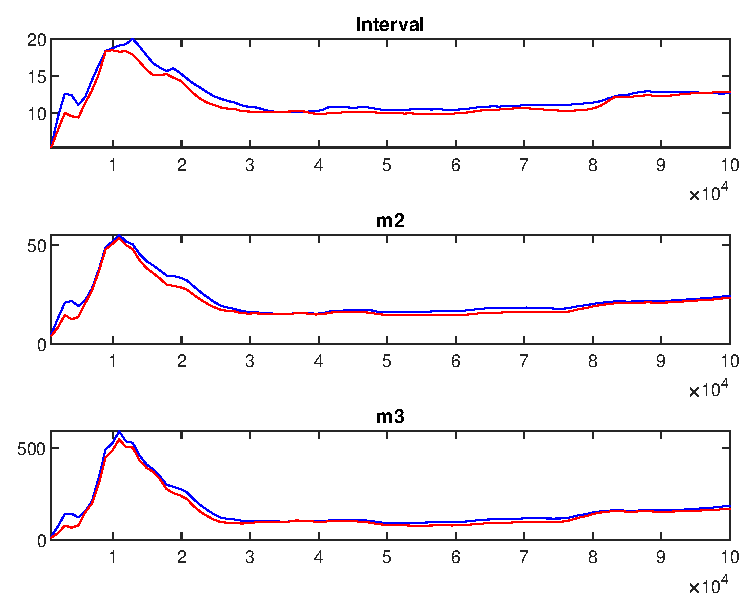
\includegraphics[width=0.8\textwidth]{GS/Output/GS_mdiag}
\caption{Multivariate convergence diagnostics for the Metropolis-Hastings.
The first, second and third rows are respectively the criteria based on
the eighty percent interval, the second and third moments. The different 
parameters are aggregated using the posterior kernel.}\label{Fig:MultivariateDiagnostics}
\end{figure}

% End Of TeX file. 
% TeX-table generated by Dynare.
% RESULTS FROM METROPOLIS HASTINGS (parameters)
% 25-Jul-2024 16:08:50 
 
\begin{center}
\begin{longtable}{llcccccc} 
\caption{Results from Metropolis-Hastings (parameters)}
 \label{Table:MHPosterior:1}\\
\toprule 
  & \multicolumn{3}{c}{Prior}  &  \multicolumn{4}{c}{Posterior} \\
  \cmidrule(r{.75em}){2-4} \cmidrule(r{.75em}){5-8}
  & Dist. & Mean  & Stdev. & Mean & Stdev. & HPD inf & HPD sup\\
\midrule \endfirsthead 
\caption{(continued)}\\\toprule 
  & \multicolumn{3}{c}{Prior}  &  \multicolumn{4}{c}{Posterior} \\
  \cmidrule(r{.75em}){2-4} \cmidrule(r{.75em}){5-8}
  & Dist. & Mean  & Stdev. & Mean & Stdev. & HPD inf & HPD sup\\
\midrule \endhead 
\bottomrule \multicolumn{8}{r}{(Continued on next page)} \endfoot 
\bottomrule \endlastfoot 
$\alpha_L$ & beta &   0.500 & 0.2500 &   0.981& 0.0094 &  0.9672 &  0.9900 \\ 
$b$ & beta &   0.710 & 0.1000 &   0.470& 0.0243 &  0.4363 &  0.5178 \\ 
$\phi$ & beta &   0.600 & 0.2000 &   0.520& 0.0175 &  0.5000 &  0.5461 \\ 
${\delta}$ & beta &   0.005 & 0.0010 &   0.015& 0.0007 &  0.0136 &  0.0156 \\ 
${1/\xi}$ & gamm &   1.000 & 0.5000 &   0.879& 0.0701 &  0.7769 &  0.9874 \\ 
${\rho_x}$ & beta &   0.600 & 0.2000 &   0.991& 0.0038 &  0.9854 &  0.9976 \\ 
${\rho_Z}$ & beta &   0.600 & 0.2000 &   0.458& 0.0272 &  0.4143 &  0.5034 \\ 
${\rho_{\alpha_L}}$ & beta &   0.600 & 0.2000 &   0.284& 0.0720 &  0.1754 &  0.3991 \\ 
${\rho_N}$ & beta &   0.600 & 0.2000 &   0.999& 0.0010 &  0.9972 &  0.9999 \\ 
\end{longtable}
 \end{center}
% End of TeX file.
 
% TeX-table generated by Dynare.
% RESULTS FROM METROPOLIS HASTINGS (standard deviation of structural shocks)
% 25-Jul-2024 16:08:53 
 
\begin{center}
\begin{longtable}{llcccccc} 
\caption{Results from Metropolis-Hastings (standard deviation of structural shocks)}
 \label{Table:MHPosterior:2}\\
\toprule 
  & \multicolumn{3}{c}{Prior}  &  \multicolumn{4}{c}{Posterior} \\
  \cmidrule(r{.75em}){2-4} \cmidrule(r{.75em}){5-8}
  & Dist. & Mean  & Stdev. & Mean & Stdev. & HPD inf & HPD sup\\
\midrule \endfirsthead 
\caption{(continued)}\\\toprule 
  & \multicolumn{3}{c}{Prior}  &  \multicolumn{4}{c}{Posterior} \\
  \cmidrule(r{.75em}){2-4} \cmidrule(r{.75em}){5-8}
  & Dist. & Mean  & Stdev. & Mean & Stdev. & HPD inf & HPD sup\\
\midrule \endhead 
\bottomrule \multicolumn{8}{r}{(Continued on next page)} \endfoot 
\bottomrule \endlastfoot 
${e_x}$ & invg &   0.010 & 0.1000 &   0.005& 0.0002 &  0.0048 &  0.0055 \\ 
${e_{b}}$ & invg &   0.010 & 0.1000 &   0.192& 0.0068 &  0.1818 &  0.2000 \\ 
${e_{alpha,L}}$ & invg &   0.010 & 0.1000 &   0.134& 0.0407 &  0.0846 &  0.1998 \\ 
${e_{\delta}}$ & invg &   0.010 & 0.1000 &   0.157& 0.0079 &  0.1438 &  0.1691 \\ 
\end{longtable}
 \end{center}
% End of TeX file.
 
% TeX-table generated by dynare_estimation (Dynare).
% RESULTS FROM POSTERIOR MAXIMIZATION (parameters)
% 25-Jul-2024 15:32:06 
 
\begin{center}
\begin{longtable}{llcccc} 
\caption{Results from posterior maximization (parameters)}\\
 \label{Table:Posterior:1}\\
\toprule 
  & \multicolumn{3}{c}{Prior}  &  \multicolumn{2}{c}{Posterior} \\
  \cmidrule(r{.75em}){2-4} \cmidrule(r{.75em}){5-6}
  & Dist. & Mean  & Stdev & Mode & Stdev \\ 
\midrule \endfirsthead 
\caption{(continued)}\\
 \bottomrule 
  & \multicolumn{3}{c}{Prior}  &  \multicolumn{2}{c}{Posterior} \\
  \cmidrule(r{.75em}){2-4} \cmidrule(r{.75em}){5-6}
  & Dist. & Mean  & Stdev & Mode & Stdev \\ 
\midrule \endhead 
\bottomrule \multicolumn{6}{r}{(Continued on next page)}\endfoot 
\bottomrule\endlastfoot 
$\alpha_L$ & beta &   0.500 & 0.2500 &   0.7182 &     NaN \\ 
$b$ & beta &   0.710 & 0.1000 &   0.4760 &     NaN \\ 
$\phi$ & beta &   0.600 & 0.2000 &   0.5873 &     NaN \\ 
${\delta}$ & beta &   0.005 & 0.0010 &   0.0170 &     NaN \\ 
${1/\xi}$ & gamm &   1.000 & 0.5000 &   0.7913 &     NaN \\ 
${\rho_x}$ & beta &   0.600 & 0.2000 &   0.9889 &     NaN \\ 
${\rho_Z}$ & beta &   0.600 & 0.2000 &   0.5102 &     NaN \\ 
${\rho_{\alpha_L}}$ & beta &   0.600 & 0.2000 &   0.1261 &     NaN \\ 
${\rho_N}$ & beta &   0.600 & 0.2000 &   0.9980 &     NaN \\ 
\end{longtable}
 \end{center}
% End of TeX file.
 
% TeX-table generated by dynare_estimation (Dynare).
% RESULTS FROM POSTERIOR MAXIMIZATION (standard deviation of structural shocks)
% 25-Jul-2024 15:32:06 
 
\begin{center}
\begin{longtable}{llcccc} 
\caption{Results from posterior maximization (standard deviation of structural shocks)}\\
 \label{Table:Posterior:2}\\
\toprule 
  & \multicolumn{3}{c}{Prior}  &  \multicolumn{2}{c}{Posterior} \\
  \cmidrule(r{.75em}){2-4} \cmidrule(r{.75em}){5-6}
  & Dist. & Mean  & Stdev & Mode & Stdev \\ 
\midrule \endfirsthead 
\caption{(continued)}\\
 \bottomrule 
  & \multicolumn{3}{c}{Prior}  &  \multicolumn{2}{c}{Posterior} \\
  \cmidrule(r{.75em}){2-4} \cmidrule(r{.75em}){5-6}
  & Dist. & Mean  & Stdev & Mode & Stdev \\ 
\midrule \endhead 
\bottomrule \multicolumn{6}{r}{(Continued on next page)}\endfoot 
\bottomrule\endlastfoot 
${e_x}$ & invg &   0.010 & 0.1000 &   0.0052 &     NaN \\ 
${e_{b}}$ & invg &   0.010 & 0.1000 &   0.1662 &     NaN \\ 
${e_{alpha,L}}$ & invg &   0.010 & 0.1000 &   0.1988 &     NaN \\ 
${e_{\delta}}$ & invg &   0.010 & 0.1000 &   0.1336 &     NaN \\ 
\end{longtable}
 \end{center}
% End of TeX file.
 
% TeX eps-loader file generated by PlotPosteriorDistributions.m (Dynare).
% 19-Jul-2024 15:55:16
 
\begin{figure}[H]
\centering
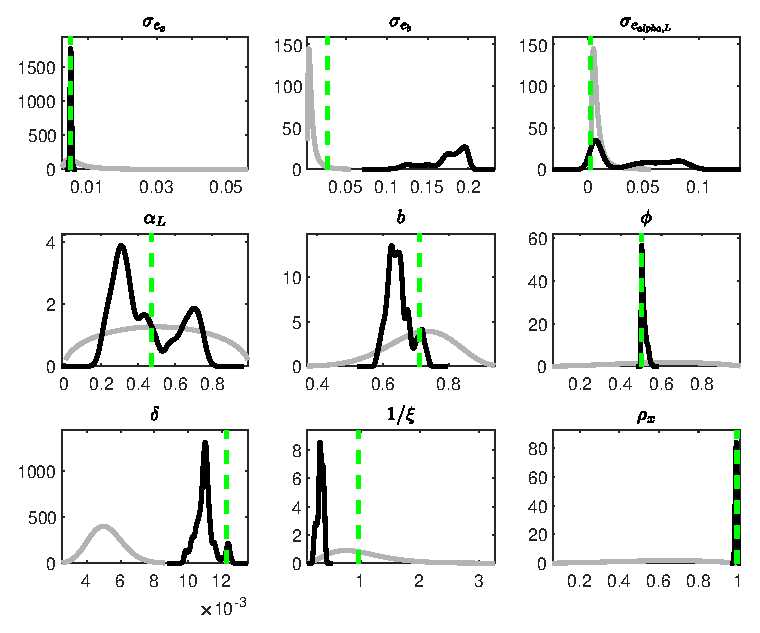
\includegraphics[width=0.80\textwidth]{GS/Output/GS_PriorsAndPosteriors1}
\caption{Priors and posteriors.}\label{Fig:PriorsAndPosteriors:1}
\end{figure}
 
\begin{figure}[H]
\centering
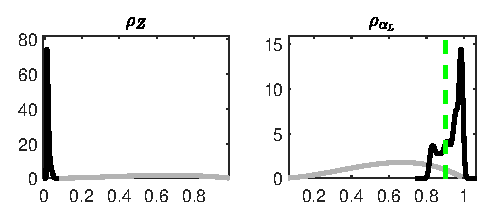
\includegraphics[width=0.53\textwidth]{GS/Output/GS_PriorsAndPosteriors2}
\caption{Priors and posteriors.}\label{Fig:PriorsAndPosteriors:2}
\end{figure}
 
% End of TeX file.
 
% TeX eps-loader file generated by McmcDiagnostics.m (Dynare).
% 25-Jul-2024 16:08:32
 
\begin{figure}[H]
\centering 
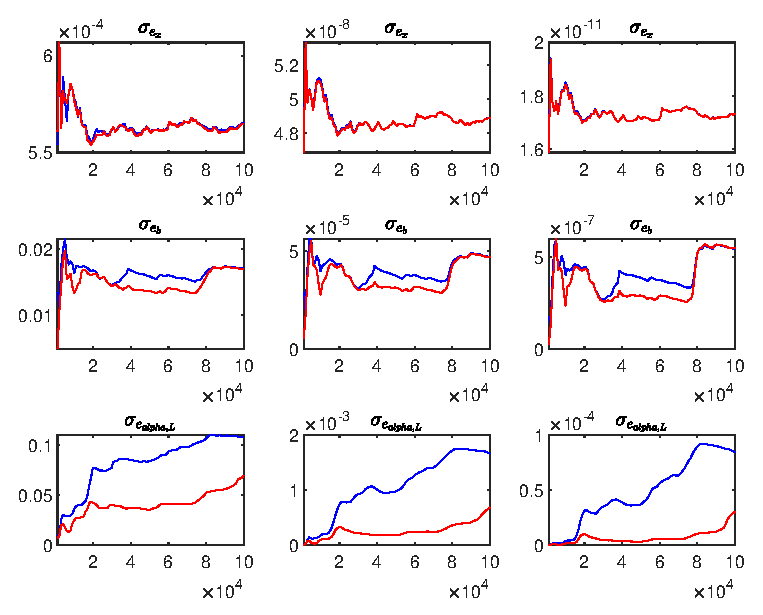
\includegraphics[width=0.80\textwidth]{GS/Output/GS_udiag1}
\caption{Univariate convergence diagnostics for the Metropolis-Hastings.
The first, second and third columns are respectively the criteria based on
the eighty percent interval, the second and third moments.}\label{Fig:UnivariateDiagnostics:1}
\end{figure}

\begin{figure}[H]
\centering 
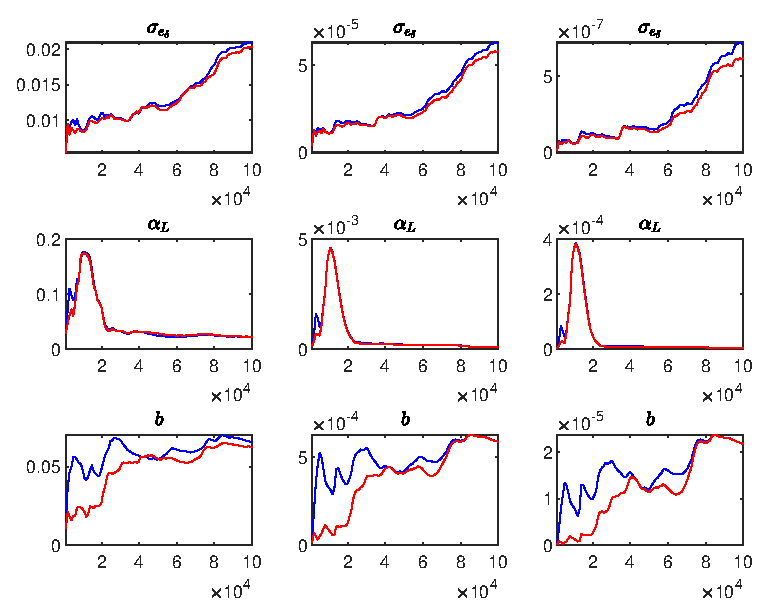
\includegraphics[width=0.80\textwidth]{GS/Output/GS_udiag2}
\caption{Univariate convergence diagnostics for the Metropolis-Hastings.
The first, second and third columns are respectively the criteria based on
the eighty percent interval, the second and third moments.}\label{Fig:UnivariateDiagnostics:2}
\end{figure}

\begin{figure}[H]
\centering 
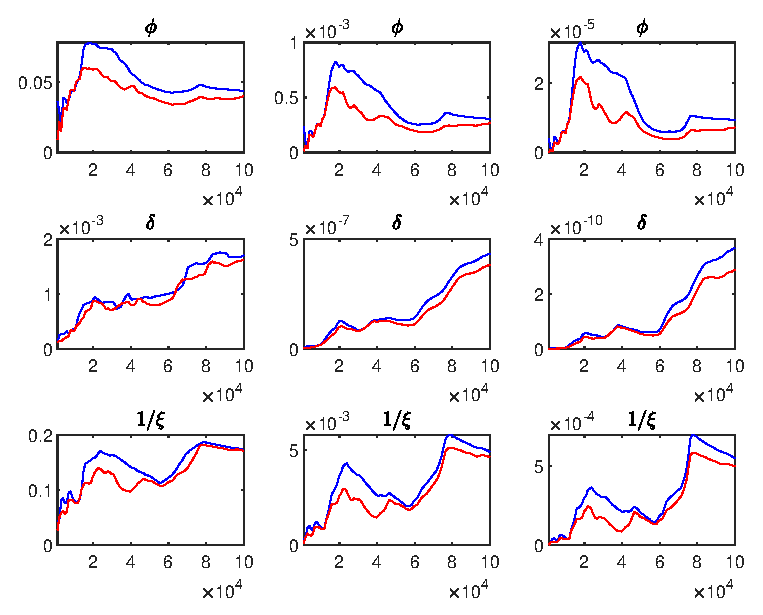
\includegraphics[width=0.80\textwidth]{GS/Output/GS_udiag3}
\caption{Univariate convergence diagnostics for the Metropolis-Hastings.
The first, second and third columns are respectively the criteria based on
the eighty percent interval, the second and third moments.}\label{Fig:UnivariateDiagnostics:3}
\end{figure}

\begin{figure}[H]
\centering 
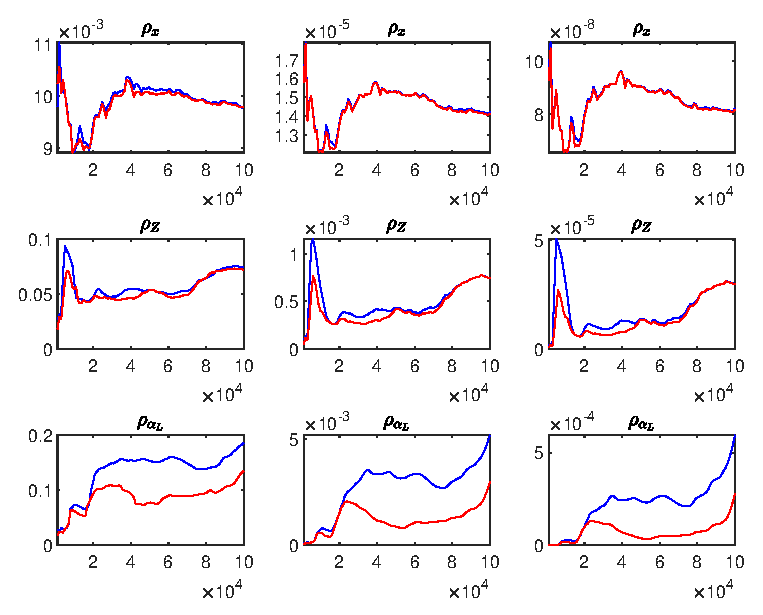
\includegraphics[width=0.80\textwidth]{GS/Output/GS_udiag4}
\caption{Univariate convergence diagnostics for the Metropolis-Hastings.
The first, second and third columns are respectively the criteria based on
the eighty percent interval, the second and third moments.}\label{Fig:UnivariateDiagnostics:4}
\end{figure}

\begin{figure}[H]
\centering 
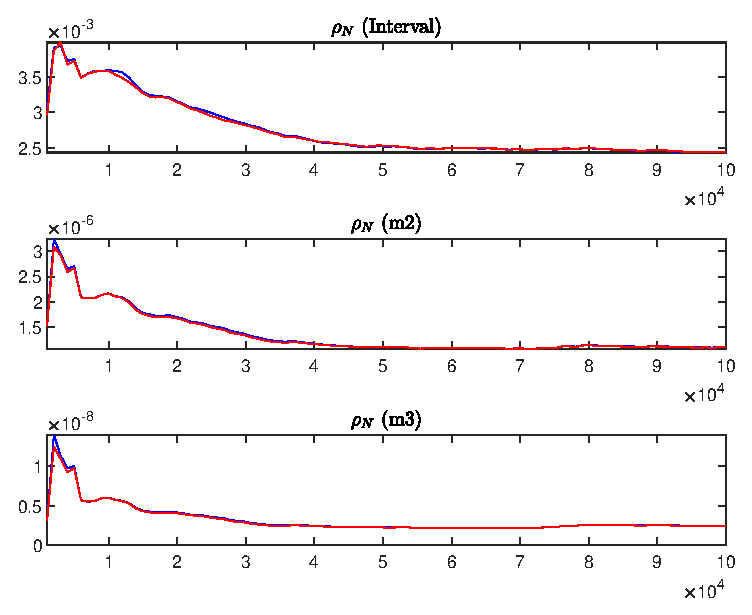
\includegraphics[width=0.80\textwidth]{GS/Output/GS_udiag5}
\caption{Univariate convergence diagnostics for the Metropolis-Hastings.
The first, second and third rows are respectively the criteria based on
the eighty percent interval, the second and third moments.}\label{Fig:UnivariateDiagnostics:5}
\end{figure}

 
% TeX eps-loader file generated by mode_check.m (Dynare).
% 25-Jul-2024 15:31:54
 
\begin{figure}[H]
\centering 
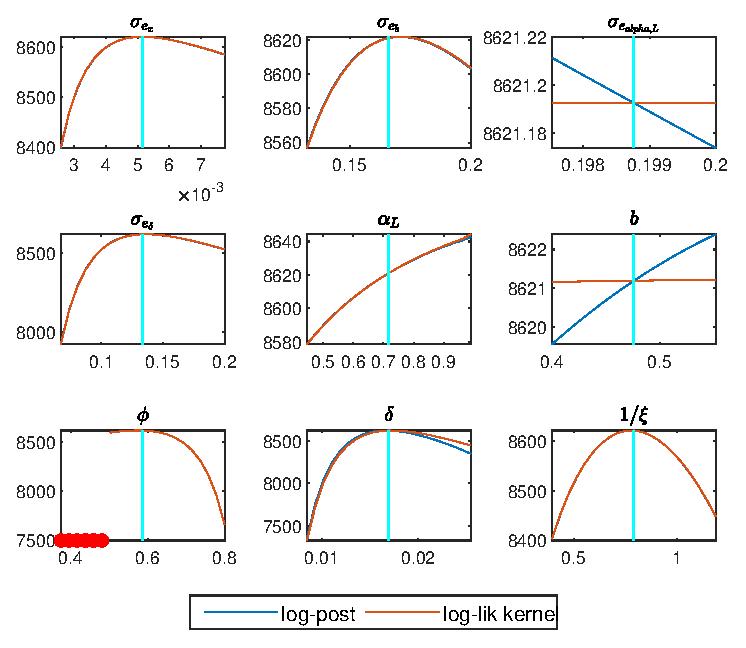
\includegraphics[width=0.80\textwidth]{GS/graphs/GS_CheckPlots1}
\caption{Check plots.}\label{Fig:CheckPlots:1}
\end{figure}
 
\begin{figure}[H]
\centering 
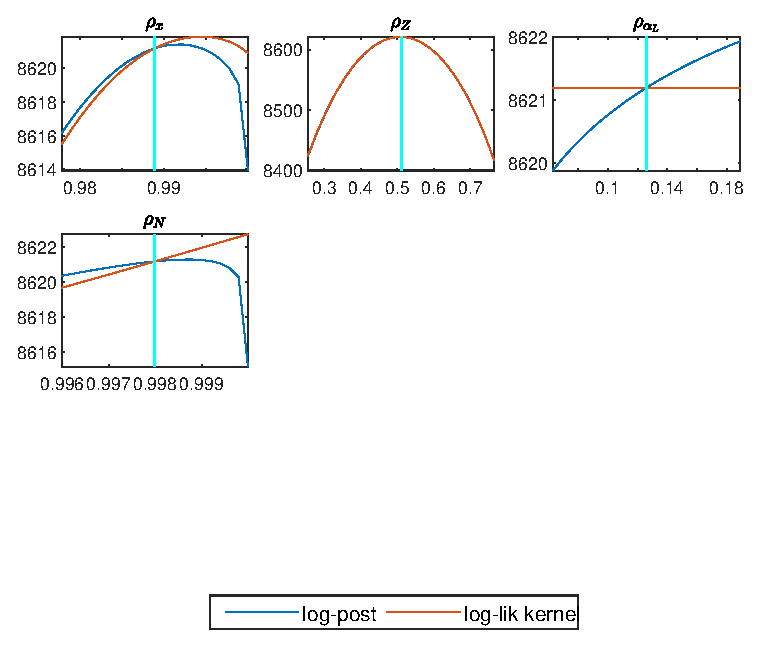
\includegraphics[width=0.80\textwidth]{GS/graphs/GS_CheckPlots2}
\caption{Check plots.}\label{Fig:CheckPlots:2}
\end{figure}
 
 
\include{GS/graphs/GS_HistoricalAndSmoothedVariables} 
% TeX eps-loader file generated by stoch_simul.m (Dynare).
% 25-Jul-2024 16:08:55
 
 
% End Of TeX file. 
 
% TeX eps-loader file generated by plot_priors.m (Dynare).
% 19-Jul-2024 15:34:48
 
\begin{figure}[H]
\centering
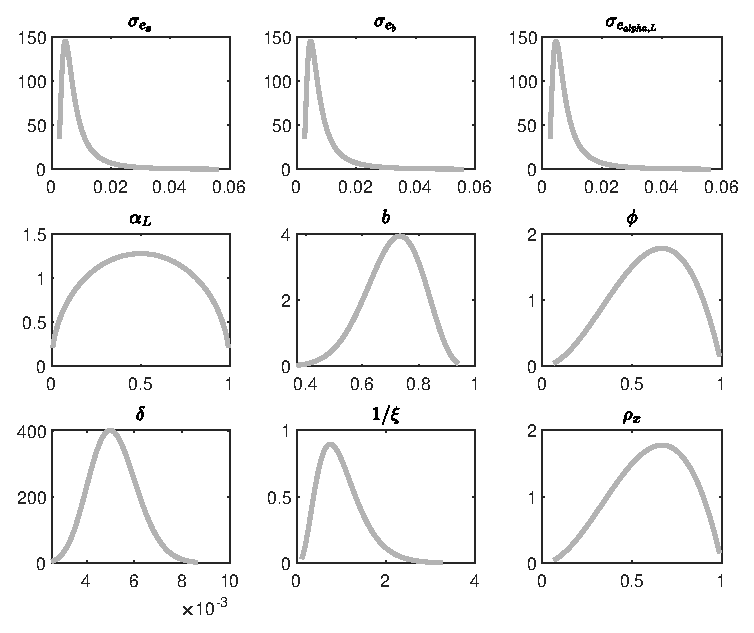
\includegraphics[width=0.80\textwidth]{GS/graphs/GS_Priors1}
\caption{Priors.}\label{Fig:Priors:1}
\end{figure}
\begin{figure}[H]
\centering
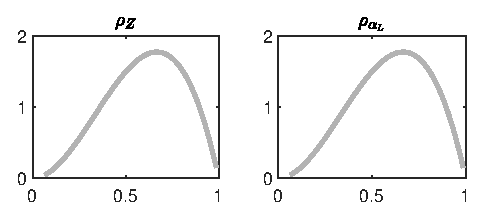
\includegraphics[width=0.53\textwidth]{GS/graphs/GS_Priors2}
\caption{Priors.}\label{Fig:Priors:2}
\end{figure}
 
% End of TeX file.
 
% TeX eps-loader file generated by dynare_estimation_1.m (Dynare).
% 19-Jul-2024 15:55:18
 
\begin{figure}[H]
\centering 
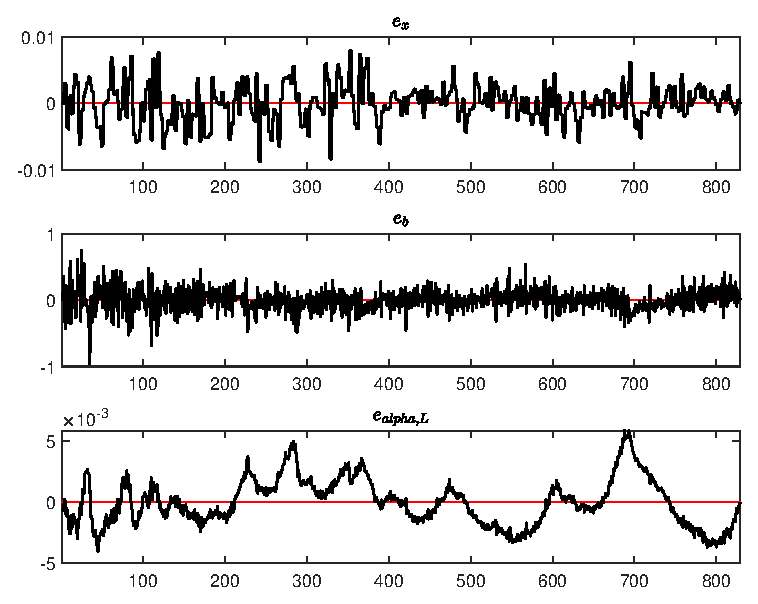
\includegraphics[width=0.80\textwidth]{GS/graphs/GS_SmoothedShocks1}
\caption{Smoothed shocks.}\label{Fig:SmoothedShocks:1}
\end{figure}


% End of TeX file.
 
\end{document} 
